 \documentclass[aps,amsfonts,amsmath,prd,preprint,nofootinbib]{revtex4}
 \pdfoutput=1
\usepackage{epsf,mathrsfs,hyperref}
\usepackage{graphicx} % To insert figures

\newcommand{\Mp}{{M_{P}}}
\newcommand{\MMp}{{M_P^2}}
\newcommand{\rmd}{{\rm d}}
\newcommand{\beq}{\begin{equation}}
\newcommand{\eeq}{\end{equation}}

\begin{document}

\title{Existence, Observers, Inference and Eternal Inflation}

\author{Richard Easther}\email{r.easther@auckland.ac.nz}
\author{Benjamin Shlaer}\email{bshl433@auckland.ac.nz} 

\address{Department of Physics, University of Auckland, Private Bag 92019, Auckland, New Zealand}



\begin{abstract}
%String theory apparently does not contain any rigorous de Sitter vacua, including meta-stable ones.  If scalar potentials supporting eternal inflation are similarly excluded \cite{Obied:2018sgi}, the multiverse, along with its anthropic solution to the dark energy magnitude problem may be in conflict with string theory.  

We consider a periodic inflection point inflationary scenario that, for some parameter values, supports  topological eternal inflation but cannot support any form of eternal inflation outside of this region of parameter space. The underlying parameter value is (in principle) measurable via the tensor-to-scalar ratio, and  the fine-tunings of the parameter values and initial conditions are strongly correlated with the total number of e-foldings.  Moreover, for parameter choices without eternal inflation scenarios the fine-tunings of the parameter values and initial conditions required for inflation to commence are strongly correlated with the total number of e-foldings.  We use this scenario as the basis for ``thought experiments'' that identify circumstances in which it would be possible to draw inferences about a cosmological multiverse scenario or anthropic resolutions of fine-tuning problems. Any such inferences will be dependent on Bayesian priors regarding the viability of the underlying model, but if eternal inflation is incompatible with quantum gravity,  seemingly fine-tuned inflationary models could stand out as islands in the swampland whereas in eternal scenarios selection effects become possible when the number of thermalized regions is large.  Finally, we note that the interpretation of Bayesian parameter estimates and model selection calculations invoke implicit assumptions about a cosmological multiverse.   

% \cite{Obied:2018sgi, Brahma:2019iyy,Kinney:2018kew}

%We consider a one-parameter space of periodic inflationary potentials, where the parameter correlates with the tensor-to-scalar ratio $r$.  For small $r$, we show that eternal inflation cannot occur regardless of initial conditions, but that it generically does occur for large $r$.  In this context, the tensor-to-scalar ratio is a proxy for the existence of a multiverse.  We examine what it means for the Planck satellite data to rule out the multiverse.  Various assumptions about the nature of observers can strongly influence our prior probability for inflationary model parameters, which may prevent meaningful model selection using CMB data alone.   We therefore comment on we should expect for the amplitude of small-scale primordial gravitational waves under various assumptions about the nature of observers.
\end{abstract}

\maketitle
\tableofcontents




\section{Introduction}


Does the CMB tell us about more than just the observable universe?  In the context of a single-field axionic inflection point model, it does.  
The way this works is that within the model class, the detection of primordial gravitational waves makes eternal inflation almost
guaranteed to have occurred.  This is because the model parameters that allow for detection of primordial gravitational waves (tensor to scalar ratio $r > 10^{-6}$) 
also require topological inflation to be eternal.  Since topological inflation occurs for any initial conditions that straddle the local maximum, the probability
for eternal inflation to occur is unity.\footnote{In any viable model, initial conditions can be tuned such that eternal inflation never occurs, although the choice may be 
difficult to justify.  For example, the inflaton can be started homogeneously from rest 70 e-folds from the bottom
of the potential.  If the initial Cauchy surface is maximal and closed, the arrow of time grows in both directions \cite{Aguirre:2007gy}, and inflation is 
past and future finite.}


Alternatively, if primordial gravitational waves can be constrained to $r < 10^{-6}$, the model does not allow for eternal inflation for any initial conditions,
and eternal inflation can be ruled out.  



The decidability of eternal inflation is not typically a feature of inflationary models.
 Observationally viable models of inflation can be always be modified to support eternal inflation before the observed final 70 e-folds.   
 For example, a local minimum can be created above the observable region of the potential $V(\phi)$.
 Aside from having a local minimum, eternal inflation can occur when
 \begin{enumerate}
 \item A region of $V$ is flat enough that a quantum fluctuations dominate over classical rolling, and so diffuse the inflaton higher up the potential, or
 \item A region of positive $V$ is wide enough in field space that gravitational self-repulsion causes a topological defect to inflate in thickness.
 \end{enumerate}
 
 Note that it is somewhat difficult to find an observationally viable potential which does not allow eternal inflation\cite{Mukhanov:2014uwa}.  (If the
potential is any polynomial, eternal inflation occurs at large field values.) %If the potential is simply unbounded above, general relativity breaks down in most of phase space.  
Conversely, just because a potential admits eternally inflating solutions (such as a quadratic potential), it may be hard to justify initial conditions with a field excursion so far away from the unique vacuum.  
Both of these make it hard to find models allowing for definitive statements about eternal inflation.

 
 
Because the number of observers apparently diverges in any theory exhibiting eternal inflation\footnote{More precisely, 
the measure problem needs to be solved to yield the fraction of observers currently making any particular observation.}, 
we will run into new challenges when considering model classes which bridge these two regions.  
For this reason, we consider here a model where the non-existence of a multiverse can be guaranteed by an observable model parameter,  the axion decay constant $f$.



A class of models that does allow strong statements about eternal inflation are axionic potentials, typically of the form \cite{shiu}
\begin{align}
V(\phi) = \sum_{j=1} c_j \exp(- m j)\left[1 + \cos(j\phi/f)\right].
\end{align}
If the field range (axion decay constant $f$) is super-Planckian, topological 
eternal inflation \cite{Vilenkin:1994pv,Linde:1994wt} occurs (see Section \ref{sec:topo}) for generic initial conditions, due to the Kibble mechanism.  
The simplest axionic model is Natural inflation \cite{freese}, but this is observationally ruled out for sub Planckian $f$.
We choose a periodic potential with an inflection point  because it is observationally viable.  
Like all smooth\footnote{In appendix \ref{sec:topo}, we show that eternal topological inflation depends only on the value of $V''/V$ at a local maximum.} periodic potentials, it can both support eternal inflation ($f \geq \sqrt{3}\Mp/2$) and exclude the possibility ($f < \sqrt{3}\Mp/2$).  
For small $f$, the last $70$ e-folds of inflation begin\footnote{
	These initial conditions are fine-tuned.  A natural mechanism to impose these initial conditions is unnecessary for our purposes, but could 
	include thermal effects which make the inflection point into a local minimum at high temperatures.}
when $\phi$ is near the inflection point \cite{Martin:2013tda, Allahverdi:2008bt, Hotchkiss:2011am,Musoke:2017frr}.



For sub-Planckian $f$, stochastic 
eternal inflation (see Appendix \ref{sec:stoc}) can occur if 
the slope of the potential is flatter than $\left|V'(\phi)\right| \lesssim \frac{3H^3}{2\pi}$ over a field range larger 
than $\Delta\phi \sim \frac{H}{2\pi}$, or if the potential has a false vacuum.
%the top of the potential resembles a quartic hilltop (or higher power).  
Hence, the simplest way to forbid eternal inflation is with a periodic potential
with sub-Planckian field range and no false vacuum.  Tuning of the slope at the inflection point allows the potential to admit 
enough e-folds to be viable, but never an infinite number.  As we show in the appendix, stochastic eternal inflation does not occur at a quadratic
local maximum of $V$ if topological eternal inflation does not occur (see Appendix \ref{app:sei}).




See also \cite{Guth:1985ya}.


The recently proposed swampland distance and de Sitter conjectures provide an example of how inflationary observables might be 
constrained by considerations from quantum gravity \cite{Brown:2015iha}.  The distance conjecture
states that any consistent effective field theory coupled to gravity is valid for a field range $\Delta\phi < {\cal D}\Mp$, which in our 
model corresponds to $f < 2\pi {\cal D}\Mp$.  The value of ${\cal D}$ depends on
the fundamental mass hierarchies \cite{Dias:2018ngv}.  The Lyth bound \cite{} then implies the upper bound $r < 8\left({\cal D}/N_{\rm tot}\right)^2$.

Similarly, the swampland de Sitter conjecture, the potential slow-roll parameter $\epsilon_V$ is bounded below by a parameter related to the mass hierarchy.
This provides  \cite{Dias:2018ngv} a bound on $r$. More...


\section{The model}
 We model the inflationary potential via
\beq
V(\phi) = \Lambda^4\left[\tfrac{4}{3\sqrt{3}}\sin(\phi/f) -\tfrac{2(1 - \beta^2)}{3\sqrt{3}} \sin(2\phi/f) + V_0  \right], \label{eq:Vp}
\eeq
where $V_0(\beta) \approx 1$ is chosen to give $V(\phi)$ a vanishing global minimum.
We will designate the parameter space for the axion decay constant as small-field ($f < \sqrt{3}\Mp/2$) or large-field ($f \geq \sqrt{3}\Mp/2$). % = \left(\frac{27 f^2 \epsilon_V(0)}{8\MMp}\right)^{1/4}\ll 1$.
The slope at the inflection point is proportional to $\beta^2$.

\begin{figure}[!h]
  \centering
    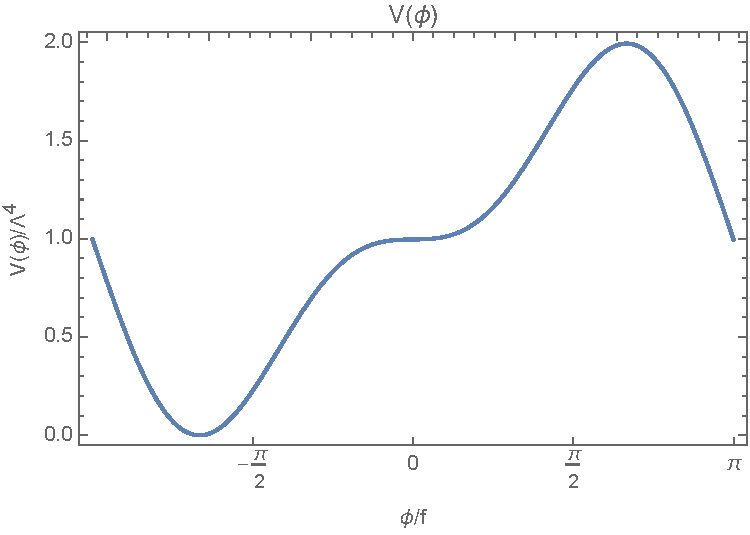
\includegraphics[width=0.5\textwidth]{figures/V.pdf}
    \caption{The potential from Eq.~(\ref{eq:Vp}).  The slope at the inflection point ($\phi = 0$) is tuned, and $f$ is a free parameter, constrained by 
    observations of the spectral index $n_s$ and the tensor-to-scalar ratio~$r$.  For $f < \sqrt{3}\Mp/2$, the potential does not allow eternal inflation regardless of initial conditions.}
\end{figure}


Inflation takes place near the inflection point at $\phi = 0$, but only if the potential is flat enough there ($\beta \ll 1$ or $f \gg \Mp$).
The field range $f$ and steepness $\beta$ are constrained by observations of the spectral index $n_s$ and tensor-to-scalar 
ratio $r$.   The scale of inflation $\Lambda$ is determined by the observed amplitude of density perturbations $A_s$.
 For large field $f/\Mp \geq \sqrt{3}/2$, topological eternal inflation generically occurs, as well as production of correspondingly large (and possibly detectable) tensor modes in the CMB.   
 For smaller $f/\Mp$ eternal inflation is impossible (see appendix \ref{sec:topo}).



\subsection{Comparison with quartic inflation}
Small-field inflation takes place very near the inflection point, in which case we can Taylor expand to cubic order about $\phi=0$. 
In this regime, we expect similar results as quartic inflation \cite{quartic}.  Musoke and Easther \cite{Musoke:2017frr} describe the general quartic model, their parametrization being related to ours by
\begin{align}
\Lambda = \frac{\sqrt[4]{\lambda } M}{\sqrt{2} \sqrt[4]{3}}, \quad f = \frac{M}{\sqrt[3]{2} \sqrt{3}}, \quad \beta = \frac{3 \sqrt{\delta}}{\sqrt[6]{2}},
\end{align}
in the small field limit $f \ll \Mp$.  Using this dictionary, we find the expected agreement between the two models in this regime.
Major differences appear in the large field regime, since our potential is periodic.  In particular, our model does not have a regime resembling $\lambda \phi^4$ inflation.  While it does
have solutions resembling quadratic hill-top inflation, we neglect these solutions for the reasons outlined below.

For $f \ll \Mp$, we will focus on solutions starting with slow roll (fine tuned) initial conditions starting at the inflection point, assuming either some mechanism can be built-in which accomplishes
this (say thermal effects which augment the potential and convert the inflection point into a local minimum of free energy), or that selection effects allow for the apparent fine-tuning of
initial conditions.

The lack of tensors seen by Planck constrains $f \leq 16\Mp$.  In the small field regime, CMB data fixes the dimensionless parameter $\beta \MMp/f^2~\sim~0.023$ which represents tuning of at least a few percent, and much more tuning for smaller $f/\Mp$.  
%Initial conditions must additionally be  tuned to about one part in ...

The scale of inflation $\Lambda^4$ does not represent significant fine-tuning, since it is a non-perturbative scale exponentially dependent on coupling constants.  
The axion decay constant $f$ is not fine tuned in this case, since it is not super Planckian.


For example, since the flatness problem is solved only by having a sufficient number of e-foldings of inflation, we argue that the (at least) percent-level tuning of parameters and initial conditions in
the small field regime could be explained as a selection effect, since structure formation requires a solution to the flatness problem.





\section{slow-roll inflation}
Inflation solves the horizon and flatness problems by proposing that a fluid with equation of state $-1< w < -1/3$ dominate the Einstein equations, allowing the co-moving Hubble distance $(a H)^{-1} = 1/\dot a$ to
shrink by a factor upwards of $e^{70}$. The most economical known example is provided by a single canonical scalar field $\phi$ dominated by its potential energy $V(\phi)$, since the quantum fluctuations of the scalar field can be the source of primordial curvature perturbations observed in the cosmic microwave background and large scale structure. 
 
The Friedmann equation and scalar equation of motion are
\begin{align}
H^2 &= \frac{1}{3\MMp}\left(\tfrac{1}{2}\dot\phi^2 + V(\phi)\right),\\
\ddot \phi &= -V'(\phi) - 3 H \dot \phi,\label{eq:scalareom}
\end{align}
where the Hubble rate is $H = \dot a/a$ and dots refer to derivatives with respect to cosmic time $t$.  


We will introduce the slow-roll approximation in the next subsection on  the small-field regime, followed by the more general
slow-roll expansion.



\subsection{Small-field regime}
In small-field models of inflation, where $\phi$ changes by much less than a Planck mass,
we must make three assumptions to obtain a viable model of inflation.  
First, the field must be initially slow, such that the potential energy dominates the Einstein equations to yield $w < -1/3$.
The Hubble friction in Eq.~(\ref{eq:scalareom}) rapidly saturates the force $V'(\phi)$, and we can neglect the $\ddot\phi$ term and solve for 
\begin{align}
\dot\phi \approx -\frac{V'(\phi)}{3 H}.
\end{align}
Thus the second assumption is that the potential is sufficiently flat to maintain $\dot\phi^2 < V$.
Finally, this must be true for at least 70 e-folds of inflation, which leads to the third assumption, 
that $V''(\phi)$ (as well as higher derivatives) must be sufficiently small in magnitude.

The second and third assumptions are captured by the smallness of the so called potential slow-roll parameters,
\begin{align}
\epsilon_V &= \frac{\MMp}{2}\left(\frac{V'(\phi)}{V(\phi)}\right)^2,\\
\eta_V &=  \MMp \frac{V''(\phi)}{V(\phi)},\\
\xi_V &= M^4_{P} \frac{V'(\phi)}{V(\phi)}\frac{V'''(\phi)}{V(\phi)}.
\end{align}
which must be $\ll 1$.

Below, we will use these parameters not just to characterize the amount of inflation, but also the spectrum
of density perturbations imprinted on the CMB.  Since these perturbations are measured on known comoving scales, we
can constrain the part of the inflationary potential where $\phi$ was rolling when the measured perturbations were generated.  Using assumptions about the
scale of reheating, we can relate comoving scale of the perturbation to the amount of inflation since that scale left the Hubble horizon.


The logarithmic change in scale factor is given by
\begin{align}
\rmd N = \frac{\rmd a}{a} = \frac{\dot a}{a\dot\phi}\rmd\phi \approx \frac{3H^2}{V'(\phi)}\rmd\phi,
\end{align}
and so the number of e-foldings $N(\phi)$ is given by
\begin{align}
N = \frac{1}{\MMp}\int \frac{V(\phi)}{V'(\phi)}\rmd\phi.
\end{align}





In the small field regime  $f < \Mp$, we can obtain a closed-form approximation for all inflationary observables.  To obtain $N_{\rm tot}$ efolds of inflation in this regime requires
\begin{align}
 \beta \leq \frac{3\pi f^2}{4\sqrt{2}\MMp~N_{\rm tot}}, 
 \end{align}
which is necessarily much less than one, since the total number of e-folds is $N_{\rm tot} \gtrsim 70$. 
which means the Hubble rate only decreases by the factor
\begin{align}
H_{\rm end}/H_{\rm start} \sim 1-\left(\frac{f}{\sqrt{6}\Mp}\right)^{3/2}
\end{align}
during inflation.  
Since $V(\phi)$ is nearly constant, 
\begin{align}
N \approx \frac{V}{\MMp}\int\frac{\rmd\phi}{V'(\phi)},
\end{align}
and we can Taylor expand $V'(\phi)$ to obtain a closed-form approximation for the value of $\phi$ corresponding to $N_\ast$ e-folds before the end of inflation:
\begin{align}
\phi_\ast/f \approx -\sqrt{\frac{2}{3}}\beta \cot\left(\frac{2\sqrt{2}\beta\MMp}{3f^2}N_\ast\right) + {\cal O}(\beta^2/\sqrt{f})
\end{align}  
This, in turn provides a closed-form solution to all of the potential slow-roll parameters
evaluated at $N_\ast$.

We find that the slow-roll parameters depend
on the parameter $\beta$ is only, to lowest order in $f/\Mp$, through the combination $\beta/f^2$.  For example, the total number of e-folds of inflation starting from the inflection point is
\begin{align}
N_{\rm tot}(\phi_{\rm i.p.}) = \frac{3 \pi f^2}{4\sqrt{2}\MMp\beta}.
\end{align}

In the small-field regime, we find the observables are well-approximated by
\begin{align}
n_s &= 1- \frac{8\sqrt{2}\beta \MMp}{3f^2\tan(\frac{\sqrt{8}N_\ast\beta\MMp}{3 f^2})},\label{eq:nsSF}\\
r &= \frac{3}{2}\left(\frac{4\beta\MMp}{3f^2\sin(\frac{\sqrt{8}N_\ast\beta\MMp}{3 f^2})}\right)^4 \left(\frac{f}{\Mp}\right)^6 ,\\
\alpha_s &= -2\left(\frac{4\beta \MMp}{3f^2\sin(\frac{\sqrt{8}N_\ast\beta\MMp}{3 f^2})} \right)^2.
\end{align}

Assuming $f < \Mp$, the spectral index constraints by Planck \cite{Akrami:2018odb} determine
\begin{align}
\frac{\beta \MMp}{f^2} = 0.023 \pm 0.001
\end{align}
 at 68\% confidence.  The degree to which the parameter $\beta$ is fine-tuned is at least a few percent, with greater tuning for smaller $f/\Mp$.


\begin{figure}[!h]
  \centering
    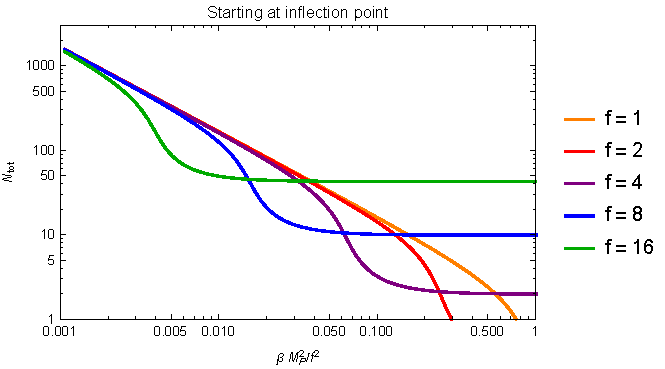
\includegraphics[width=0.7\textwidth]{figures/NvsBetaf-2.pdf}
    \caption{The total number of e-folds for inflation beginning at the inflection point.  In the small-field regime, the number of e-folds depends only on the ratio $\beta \MMp f^{-2}.$}
\end{figure}



\begin{figure}[!h]
  \centering
    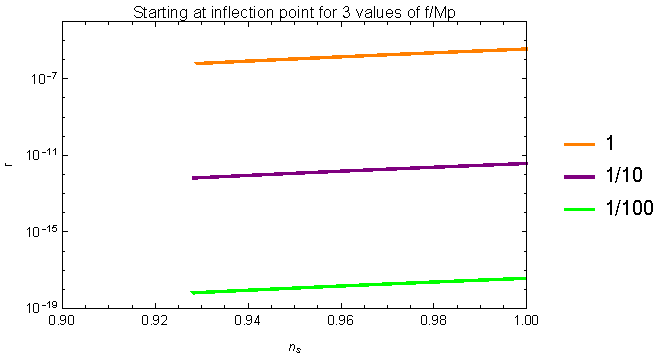
\includegraphics[width=0.7\textwidth]{figures/rvsnsplot.pdf}
    \caption{The tensor-to-scalar ratio in the small field regime.  $N = 55$ e-folds.}
\end{figure}




\begin{figure}[!h]
  \centering
    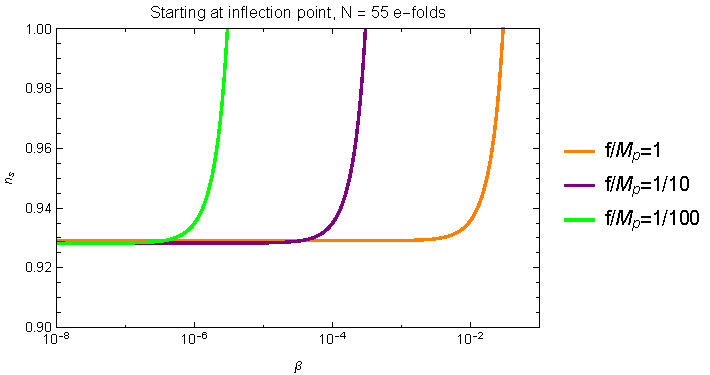
\includegraphics[width=0.7\textwidth]{figures/nsvsbetaplot2.pdf}
    \caption{The spectral index in the small field regime.}
\end{figure}

\begin{figure}[!h]
  \centering
    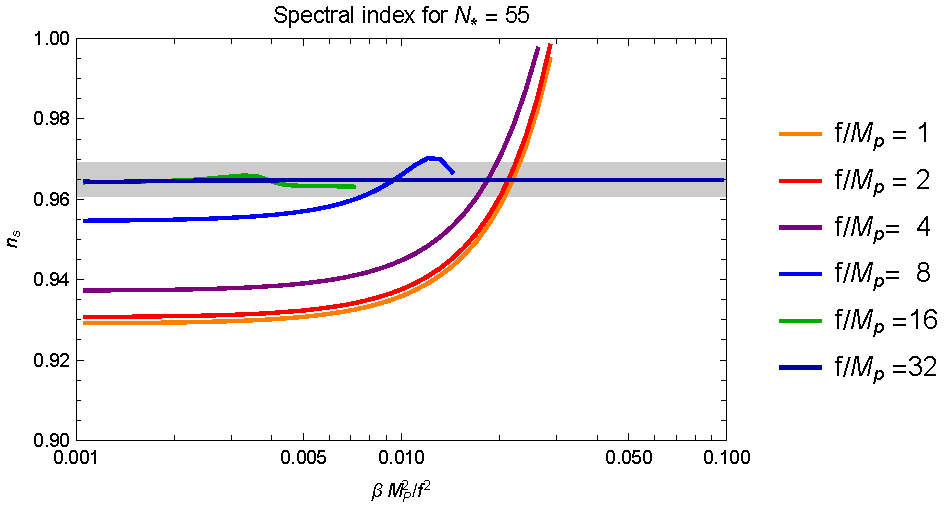
\includegraphics[width=0.7\textwidth]{figures/nsvsb.pdf}
    \caption{The spectral index in the large field regime. The endpoints of the lines for the largest two values of $f$ correspond to where less than 55 e-folds of inflation occur.
    Note that in the small field ($f < \Mp$) regime, $n_s$ depends only on $\beta \MMp f^{-2}$.}
\end{figure}

\begin{figure}[!h]
  \centering
    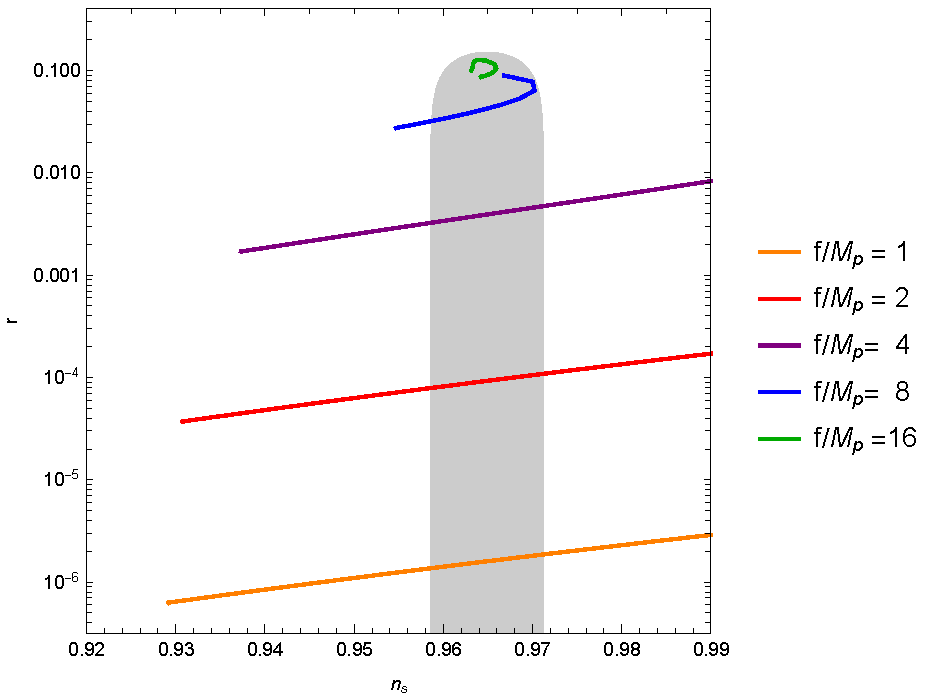
\includegraphics[width=0.6\textwidth]{figures/nsrplotvsf.pdf}
    \caption{The tensor to scalar ratio vs. spectral index in the large field regime.  The left endpoints correspond to $\beta = 0$, while the right endpoints correspond to less than 55 e-folds of inflation.}
\end{figure}

\begin{figure}[!h]
  \centering
    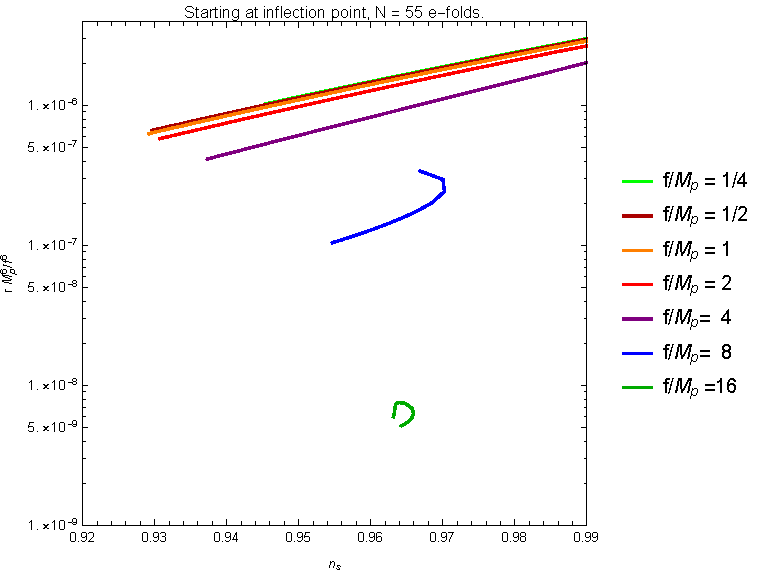
\includegraphics[width=0.6\textwidth]{figures/nsrf6plotvsf.pdf}
    \caption{The rescaled tensor to scalar ratio vs. spectral index. Note that in the small field regime, $r (\Mp/f)^6$ is dependent only on $\beta$ through the combination $\beta/f^2$, as seen in Eq.~(\ref{eq:nsSF}).}
\end{figure}




\begin{figure}[!h]
  \centering
    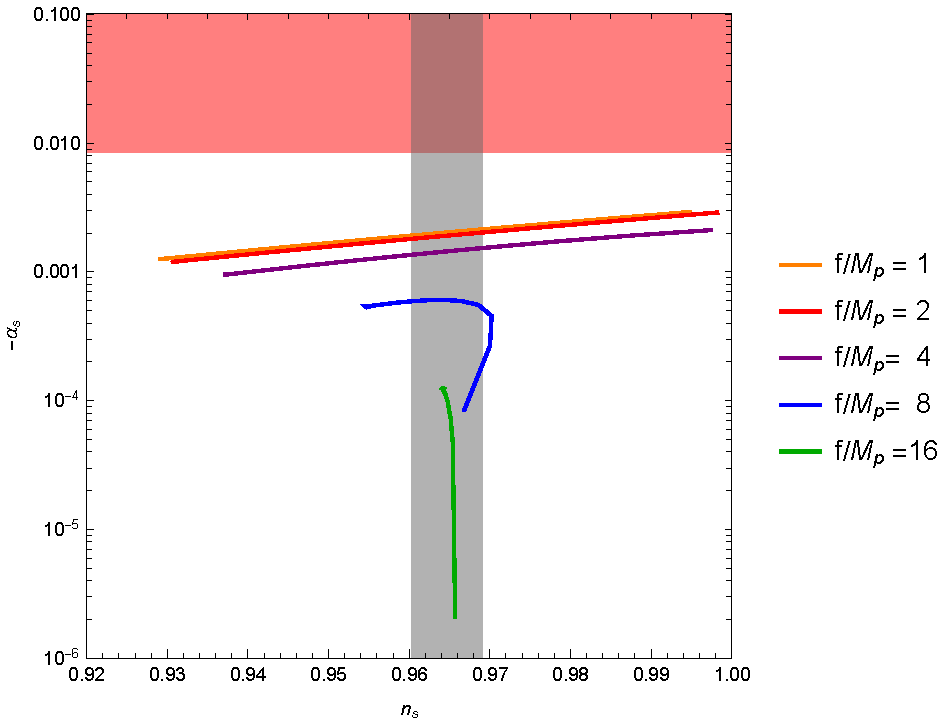
\includegraphics[width=0.7\textwidth]{figures/alphasvsnsplot.pdf}
    \caption{The running of the spectral index in the small field regime.  $N = 55$ e-folds.}
\end{figure}





\begin{figure}[!h]
  \centering
    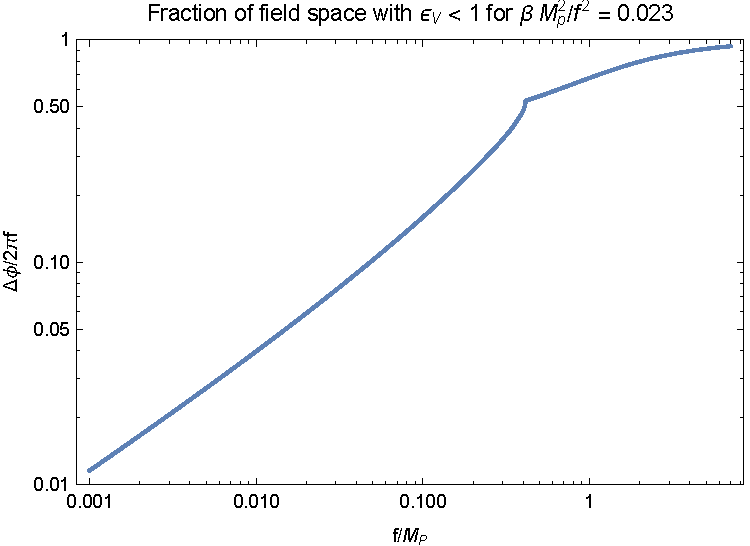
\includegraphics[width=0.7\textwidth]{figures/SRfraction.pdf}
    \caption{The fraction of field space where inflation can take place.  Smaller values of $f$ require more fine-tuned initial field values, unless a 
    mechanism is used to deform a local minimum into the inflection point, either
    as a function of temperature or other fields.  For the observationally viable value of $\beta$ used here, the initial inflaton displacement must be fine-tuned by the factor $\Delta\phi/(2\pi f) \approx \sqrt{f/\Mp}$ in the small field regime.}
\end{figure}







\subsection{More general formalism}


We follow the Hubble slow-roll formalization of \cite{Liddle:1994dx}.  


Taking a time derivative of the Friedmann equation 
and eliminating $\ddot \phi$ using the scalar equation of motion results in
\begin{align}
\dot H = -\frac{\dot \phi^2}{2\MMp}.
\end{align}
Dividing this expression by $\dot\phi$ yields
\begin{align}\label{eq:phidot}
H'(\phi) = -\frac{\dot \phi}{2\MMp},
\end{align}
which allows us to eliminate $\dot \phi$ and instead use
the inflaton $\phi$ as a time variable during inflation, when $\phi_i \leq \phi \leq \phi_f$.  The Friedmann equation becomes
\begin{align}\label{eq:Heom}
H'(\phi)^2 = \frac{3 H^2(\phi)}{2\MMp} - \frac{V(\phi)}{2 M^4_P},
\end{align}
with initial condition
\begin{align}
H(\phi_i) = \sqrt{\frac{1}{3\MMp}\left[\tfrac{1}{2}\dot \phi_i^2 + V(\phi_i)  \right]}.
\end{align}
We numerically integrate\footnote{For numerical stability, we integrate the equivalent equation $T'(\phi) = \sqrt{6T\left(T+V\right)}/\Mp - V'(\phi)$, where $T(\phi) = 3\MMp H^2(\phi) - V(\phi)$ is the kinetic energy density of the inflaton.}
the Friedmann equation (\ref{eq:Heom}) using the (approximate) attractor initial condition ${\dot \phi_i = -V'(\phi_i)/[3H(\phi_i)]}$.  Inflation ends when the 
comoving Hubble distance $\left(a H\right)^{-1}$ stops decreasing, i.e. when ${\ddot a(t) \leq 0}$.  This moment defines $\phi_f$. 

The Hubble slow-roll parameters are defined by
\begin{align}
\epsilon_H &= 2\MMp \left(\frac{H'(\phi)}{H(\phi)}\right)^2,\\
\eta_H &= 2\MMp \frac{H''(\phi)}{H(\phi)},
\end{align}
and so the end of inflation also coincides with ${\epsilon_H(\phi) \to 1}$.  

The remaining number of e-foldings between $\phi$ and $\phi_f$ is defined by the ratio of comoving Hubble distances, 
\begin{align}
N(\phi) = \ln\left(\frac{a(\phi_f) H(\phi_f)}{a(\phi) H(\phi)}\right),
\end{align}
which we compute by numerically integrating:
\begin{align}
N(\phi) = \frac{1}{\sqrt{2\MMp}}\int_{\phi}^{\phi_f} \frac{1-\epsilon_H(\phi)}{\sqrt{\epsilon_H(\phi)}}\rmd \phi .
\end{align}


\subsection{Perturbations}
The amplitude of the inflaton perturbation on a given comoving scale $k$ is given by the Hubble rate when that
scale exits the Hubble ``horizon.''   The inflaton perturbation is also a perturbation in the time of reheating, after which it is converted to a density perturbations with
amplitude
\begin{align}
{\cal P}_{\cal R}^{1/2}(k) \approx \left.\frac{H^2(\phi)}{2\pi|\dot\phi|}\right|_{k = a H}.
\end{align}
Here the classical field velocity $\dot\phi$ and Hubble rate $H$ are evaluated at the moment when the comoving length scale of interest $1/k$ crosses the monotonically decreasing ``horizon'' $(aH)^{-1}$.
This spectrum of density perturbations is observed in the CMB to be well characterized by the amplitude $A_s$, spectral index $n_s$, and running $\alpha_s$ and via
\begin{align}
 {\cal P}_{\cal R}(k) = A_s(k_\ast)\left(\frac{k}{k_\ast}\right)^{n_s - 1 + \frac{\alpha_s}{2}\ln(k/k_\ast) + ...}
\end{align}

A similar expression holds for tensor perturbations, 
\begin{align}
{\cal P}_{t}^{1/2}(k) \approx \left.\frac{H^2(\phi)}{2\pi\MMp}\right|_{k = a H},
\end{align}
but we will only be interested in the tensor to scalar ratio
\begin{align}
r = \frac{A_t(k_\ast)}{A_s(k_\ast)}.
\end{align}


\subsection{observables}
Primordial perturbations at each comoving scale directly 
generate (via a cosmological model like $\Lambda_{\rm CDM}$) CMB and large-scale structure observables.   In the case of single-field inflation, these primordial perturbations can 
be described entirely by the Hubble rate and Hubble slow-roll parameters.

The quantum fluctuation of both the metric and inflaton on a given comoving scale $k$ are generated when the wavelength is stretched beyond the Hubble distance, $(a H)^{-1}$.
Since the comoving Hubble distance decreases monotonically during inflation, we can relate each comoving scale $k$ to a single value of $\phi$ (and thus $N(\phi)$). 
\begin{align}
N(\phi) \longleftrightarrow \phi \longleftrightarrow k = a(\phi) H(\phi).
\end{align}  



 

We may express the slow-roll parameters either as a function of $\phi$, as a function of $N$,
or as a function of $k$, the latter being more directly related to CMB angular scales.  
The amplitude of curvature perturbations on comoving scale ${k = a(\phi) H(\phi)}$ is \cite{Stewart:1993bc}
\begin{align}
{\cal P}_{\cal R}^{\frac{1}{2}}(k) = 2^{\nu - \tfrac{3}{2}}\frac{\Gamma(\nu)}{\Gamma(\tfrac{3}{2})}\left[1-\epsilon_H(\phi)\right]^{\nu - \tfrac{1}{2}}\left.\frac{H^2(\phi)}{2\pi|\dot\phi|}\right. , 
\end{align}
where $\nu = \frac{1+\epsilon_H(\phi) - \eta_H(\phi)}{1-\epsilon_H(\phi)} + \frac{1}{2}$, and $\dot \phi$ can be solved for using equation (\ref{eq:phidot}).
Then the measured amplitude at an arbitrarily chosen pivot scale $k_\ast = a(\phi_\ast) H(\phi_\ast)$ is given by
\begin{align}
A_s = {\cal P}_{\cal R}(k_\ast) .
\end{align}
Near the pivot scale, we can characterize the power spectrum of scalar perturbations by essentially its first three Taylor coefficients, $A_s, n_s, $ and $\alpha_s$ via
\begin{align}
 {\cal P}_{\cal R}(k) = A_s(k_\ast)\left(\frac{k}{k_\ast}\right)^{n_s - 1 + \frac{\alpha_s}{2}\ln(k/k_\ast) + ...}
\end{align}
A similar expansion holds for tensor perturbations, but we will only be interested in the tensor to scalar ratio
\begin{align}
r = \frac{A_t(k_\ast)}{A_s(k_\ast)}.
\end{align}

The scalar spectral index, tensor-to-scalar ratio, and scalar running are given in terms of the slow-roll parameters up to 2nd order by \cite{Easther:2006tv}
\begin{align}
n_s &= 1 - 4\epsilon_H + 2\eta_H - 2(1+{\cal C})\epsilon_H^2 - \frac{1}{2}(3-5{\cal C})\epsilon_H\eta_H + \frac{1}{2}\left(3-{\cal C}\right)\xi_H ,\\
r &= 16\epsilon_H\left[1+2{\cal C}(\epsilon_H-\eta_H)  \right],\\
\alpha_s &= \frac{-1}{1-\epsilon_H}\left( 2\xi_H-8 \epsilon_H^2 - 10 \epsilon_H\eta_H  + \frac{7{\cal C}-9}{2}\epsilon_H\xi_H + \frac{3-{\cal C}}{2}\eta_H\xi_H\right),
\end{align}
where ${\cal C} = 4(\ln 2 + \gamma_E)-5$.
Since $n_s(\phi_\ast)$, $r(\phi_\ast)$, and $N(\phi_\ast)$ only depend on the shape of the potential and are independent of the scale of inflation, $\Lambda$,
we can fix $\Lambda$ via measurements of $A_s$ without significantly affecting $n_s$ and $r$.
(A small dependence of $n_s$ and $r$ on $\Lambda$ is introduced since the value of $\phi_\ast$ when they are measured does have logarithmic dependence on $\Lambda$, roughly corresponding
to $50 \lesssim N_\ast \lesssim 60$.)

%We completely fix $\Lambda$ by the scalar amplitude $A_s$.

\subsection{Fine tuning of parameters}
Our results are similar to those found in \cite{Musoke:2017frr}, which considered inflection point inflation in a quartic potential.  In particular, for $f = \Mp/10$, the slope parameter at the inflection point, $\beta$, must be
tuned to be about $10^{-4}$ in order to satisfy the Planck constraints on both $n_s$ and $\alpha_s$.  The scale of inflation $\Lambda$ must additionally be tuned, although a technically-natural mechanism exists for axion-like (periodic) potentials.  Finally, the initial conditions are also tuned to a high degree, as generic initial conditions lead to the overshoot problem.

The situation appears better for large field inflation.
For $f = 10 \Mp$, there is far less tuning necessary, except for the implied suppression of couplings to all UV degrees of freedom that normally forbid super-Planckian field excursions \cite{swampland, monodromy}.

For $f > 100 \Mp$, the model is indistinguishable from chaotic $m^2\phi^2$ inflation, running into  

The main constraint in this case comes from observations indicating the tensor-to-scalar ratio obeys $r \lesssim 0.06$.

Without considering the implications of eternal inflation on the number of observers, the question of what the true value of $f$ is 


\begin{figure}[!h]
  \centering
    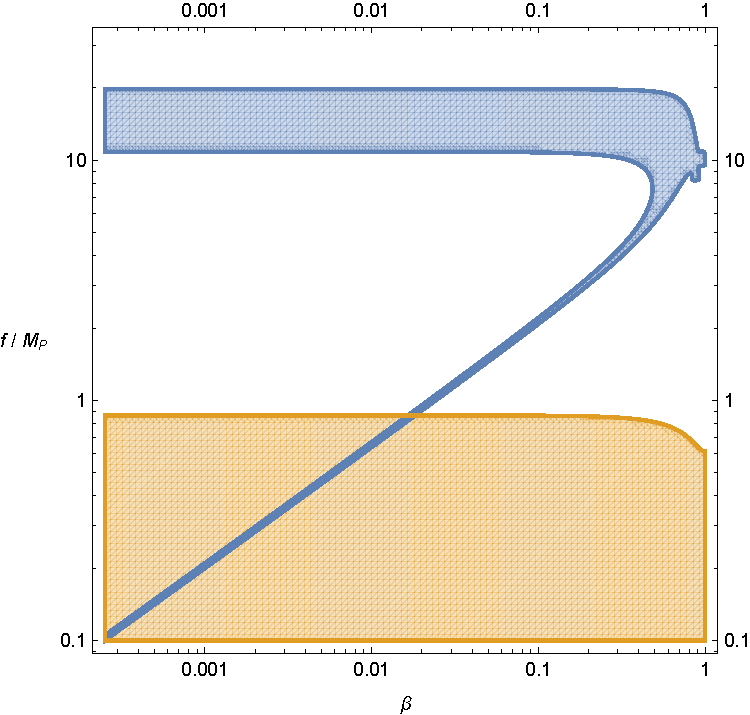
\includegraphics[width=0.7\textwidth]{figures/fbregionPlanck2018.pdf}
    \caption{The fraction of parameter space compatible with Planck 2018 (blue).  The region where eternal inflation is impossible is shaded in orange.}
\end{figure}












\subsection*{Acknowledgements}
This work was supported by a grant from the Foundational Questions Institute (FQXi).




\begin{appendix}










\section{Topological Eternal Inflation}\label{sec:topo}
Topological eternal inflation \cite{Vilenkin:1994pv,Linde:1994wt} occurs when the gravitational repulsion sourced by a topological defect causes the breakdown of any static finite thickness solution containing a defect.  Instead, 
the thickness of any topological grows exponentially.  It typically \cite{Sakai:2003st}
occurs when the vacuum manifold is larger than the Planck mass in field space.  

We will quantify the onset of topological eternal inflation by considering the stability of the classical de Sitter solution with homogeneous scalar field at the top of the potential.  When a perturbation about this
solution exists which is both
\begin{enumerate}
\item unstable
\item of nonzero topological charge
 \end{enumerate}
 we claim that the topological inflation is then and only then not eternal.
Because we are considering a single-field inflationary model, the only topological defects that may exist are domain walls.  %The topological charge of a perturbation in this case is $(-1)^{\text{\# of nodes}}$.





\subsection{Domain wall geometry}
One should expect that a positive tension domain wall would be gravitationally repulsive, owing to the concept of active gravitational mass.  Furthermore, 
the gravitational repulsion should be position-independent far from the core of the defect, since the Green's function for a co-dimension one Newtonian
source is a linear potential.  Position-independent repulsion means the spacetime surrounding a domain wall should be flat, with the domain wall accelerating away from any inertial observer.  
For example, an expanding bubble in Minkowski space appears repulsive to observers inside the bubble.  Thus we are led to the ISV ansatz
of a domain wall as two copies of the interior of a bubble geometry, glued together on the surface of the bubble, as seen in the left-hand panel of Figure~\ref{fig:ISV}.
\begin{figure}[htbp]
\begin{center}
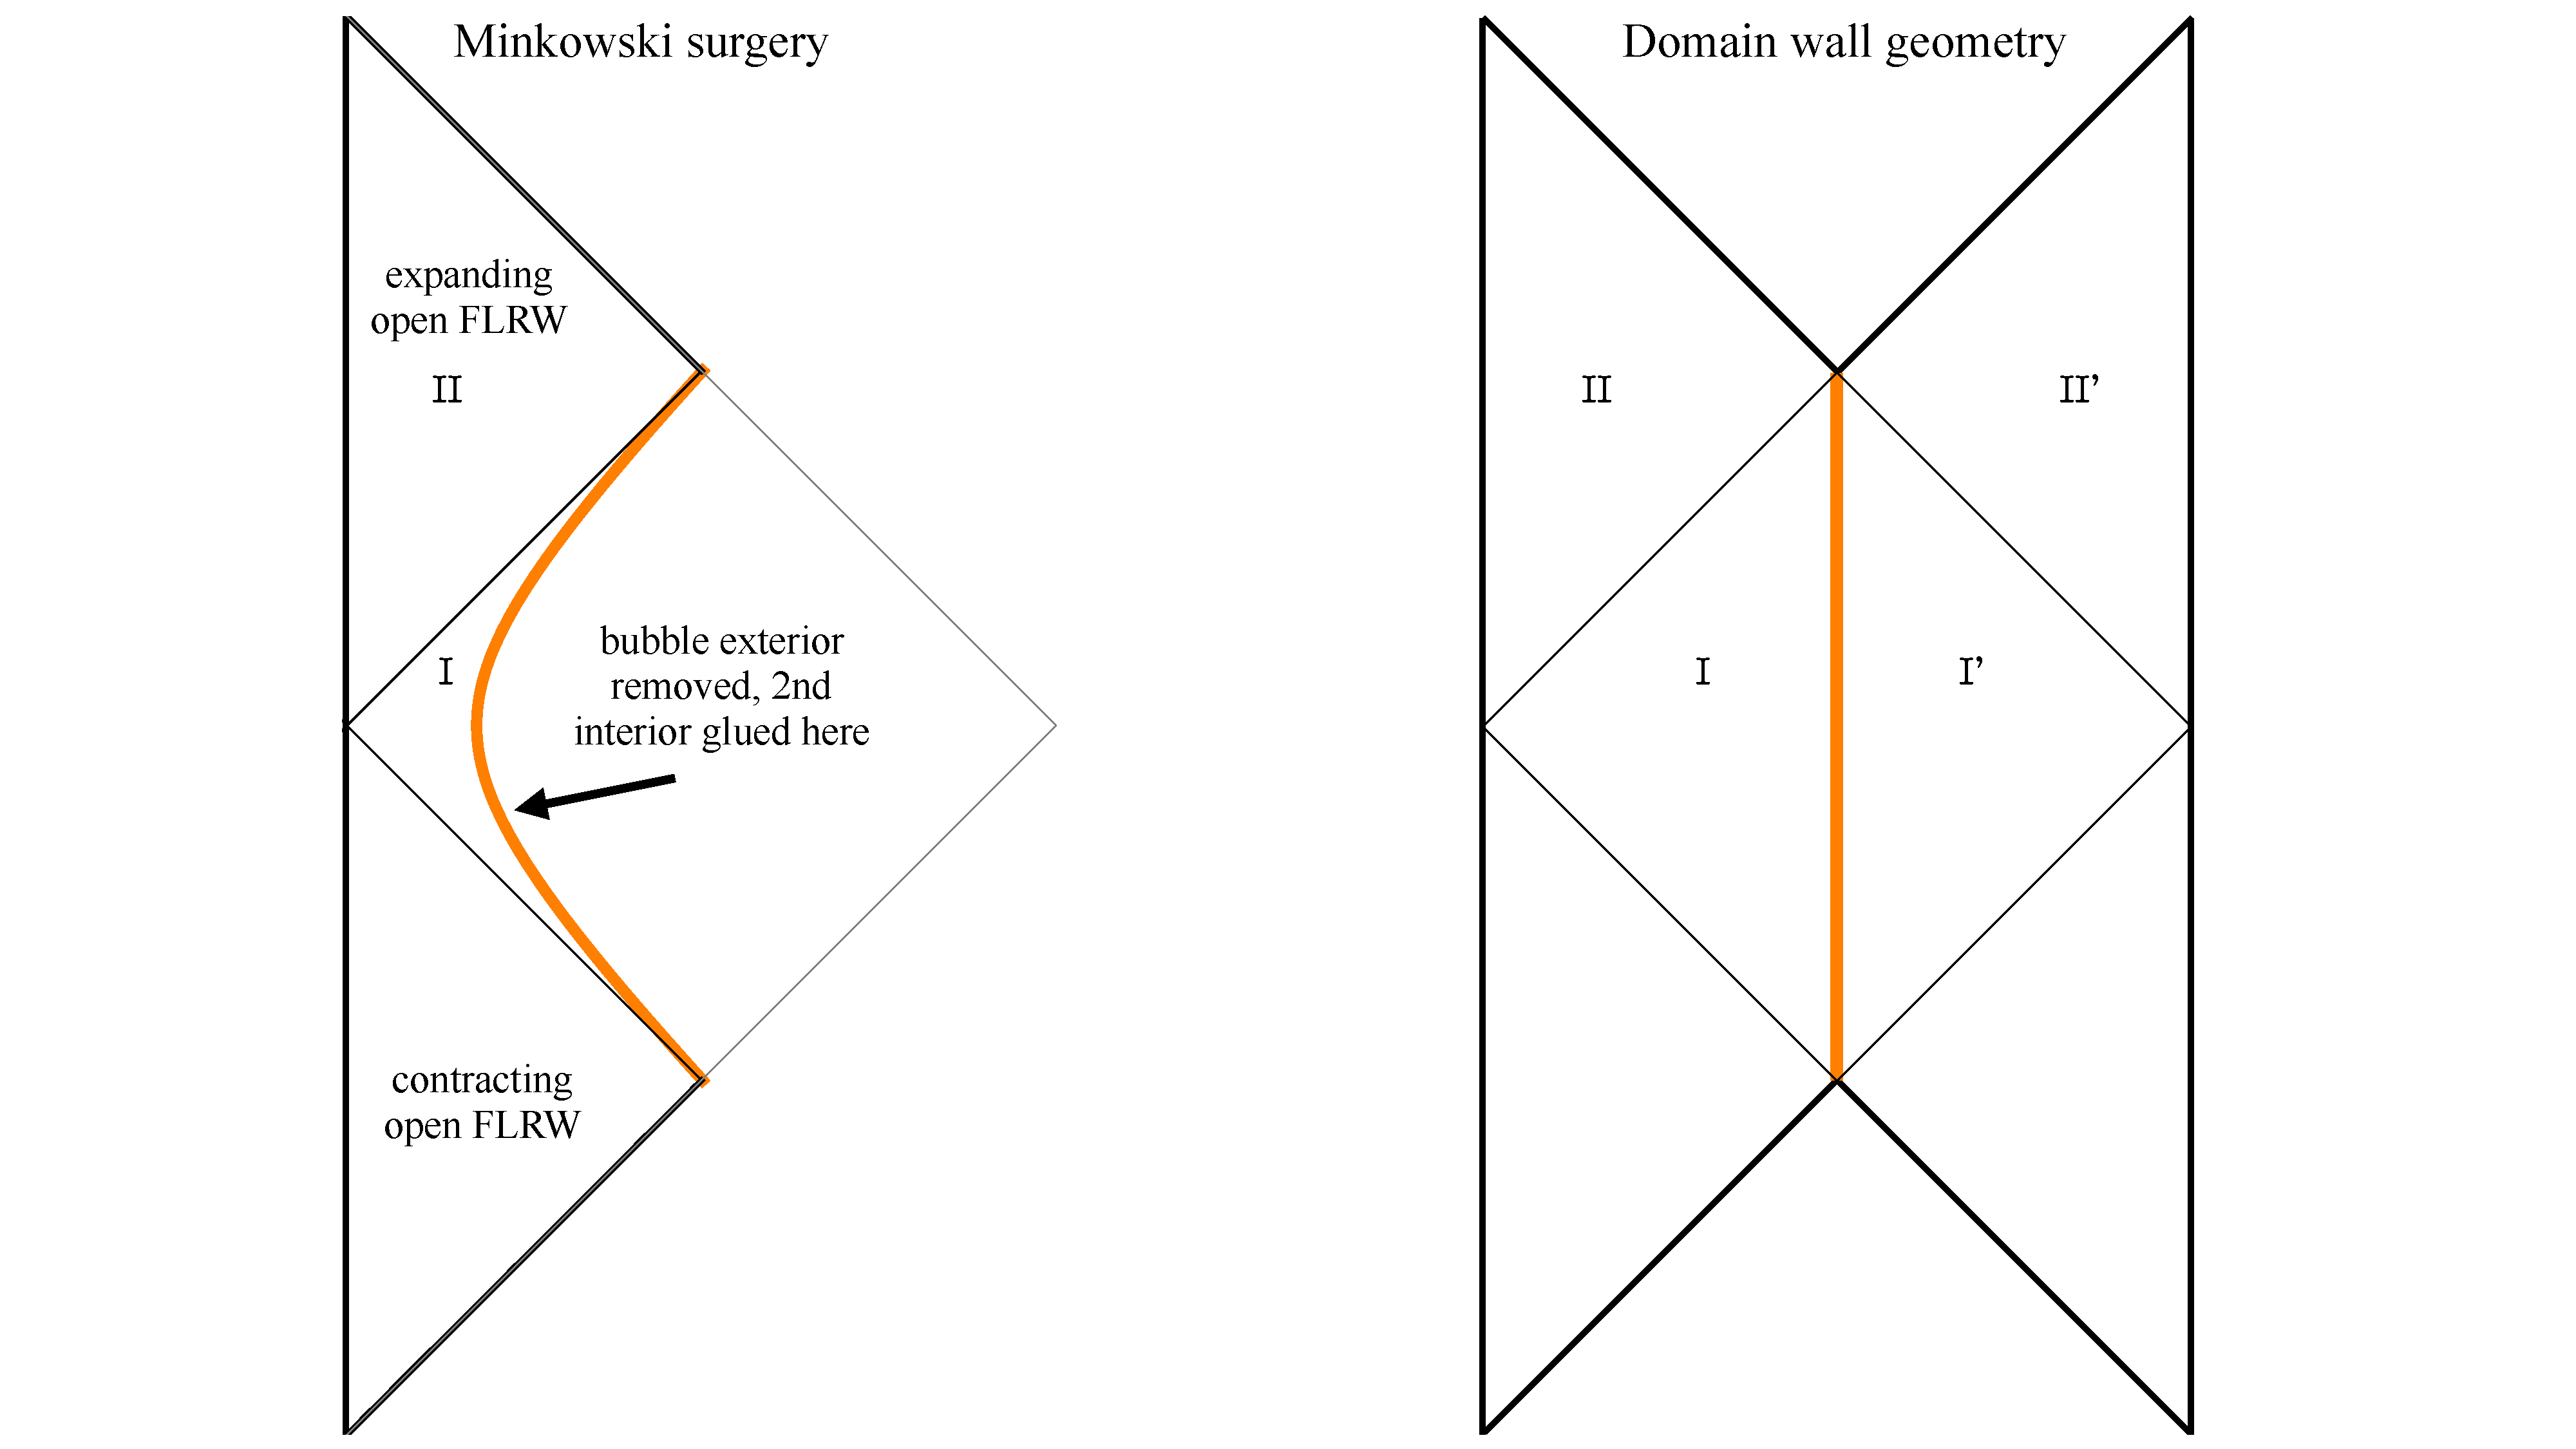
\includegraphics[width=1\textwidth]{figures/ISVbubble}
\caption{{\bf Left:} The ground state domain wall geometry consists of two copies of the interior of a bubble in Minkowski space.    {\bf Right:} They are glued together on the defect core (orange represents energy density). 
The metric in Eq.~(\ref{eq:ISVmetric}) only covers the interior regions I and I', between the four horizons (two future and two past), where $\ell(z_h^\pm) = 0$.  This includes the core, where $\dot\ell(0) = 0$. The future open FLRW regions (II, II') are obtained by
double analytic continuation $z\to i t$, $t \to r + i\pi/2$ of the metric in Eq.~(\ref{eq:ISVmetric})}.
\label{fig:ISV}
\end{center}
\end{figure}


The metric sourced by a static ``planar'' domain wall has the ISV \cite{Ipser:1983db, Vilenkin:1984hy} form
\begin{align}
\rmd s^2 = \rmd z^2 + \ell^2(z)\left( -\rmd t^2 + \cosh^2 t~\rmd \Omega_2^2\right),\label{eq:ISVmetric}
\end{align}
i.e. it can be described as a nested family of 2+1 dimensional global de Sitter slices.  The scalar field is a function only of the transverse coordinate $z$, as is the curvature radius of the 2+1 dimensional de Sitter slice
given by $\ell(z)$.  For a thin domain wall, $\ell(z)$ rises and falls with unit magnitude slope, curving over at the peak due to the energy density.  There is a future and past horizon at each of the two roots, $\ell(z_h^\pm) = 0$, across each of which the geometry is a non-singular open FLRW big-crunch/big-bang universe.



\subsection{Onset of topological eternal inflation}
In the coordinate patch centered on the domain wall core and extending to the horizons on either side,
the unperturbed eternally inflating ``domain wall'' appears homogeneous, taking the exact de Sitter form
\begin{align}
\phi(t,z) = \phi_{\rm peak}, \qquad \ell(z) = \ell_0\cos\left(z/\ell_0 \right),
\end{align}
where $\ell_0 = \sqrt{\frac{3}{V(\phi_{\rm peak})}}\Mp$.   

A ``monopole'' perturbation $\delta\phi$ (meaning one which has no nodes, e.g., $\delta\phi \geq 0$) causes a thermalized region to form.  However, a ``dipole'' perturbation
(meaning one which vanishes along some co-dimension one surface, say $z=0$) is topologically prevented from homogeneously rolling to the vacuum.  Instead, two thermalized regions form separated by a domain wall.
In the non-eternally inflating regime of parameter space, the thermalized regions are separated by static, finite thickness domain walls.  

In the eternally inflating regime, perturbations still lead to thermalized pocket universes, but the domain walls separating them are not static, but rather growing in thickness.
While the thermalized regions fall through the horizons, the homogeneous de Sitter solution remains valid in the interior region of our soliton-centered coordinate patch.
In other words, for topological eternal inflation, the de Sitter maximum is stable under perturbations with a node at $z = 0$.  

The longest wavelength (fastest growing) perturbation with a
node at $z=0$ is given by $\delta\phi \propto \sin(z/\ell_0)$, since the equations of motion require $\partial_z\phi$ to vanish at the horizons, where $z = \pm \pi \ell_0/2$.
This perturbation grows when topological inflation is not eternal, but decays back to a homogeneous de Sitter patch when it is eternal.
Thus the threshold for topological eternal inflation occurs when this longest wavelength mode is static, neither growing nor decaying.


\begin{figure}[htbp]
\begin{center}
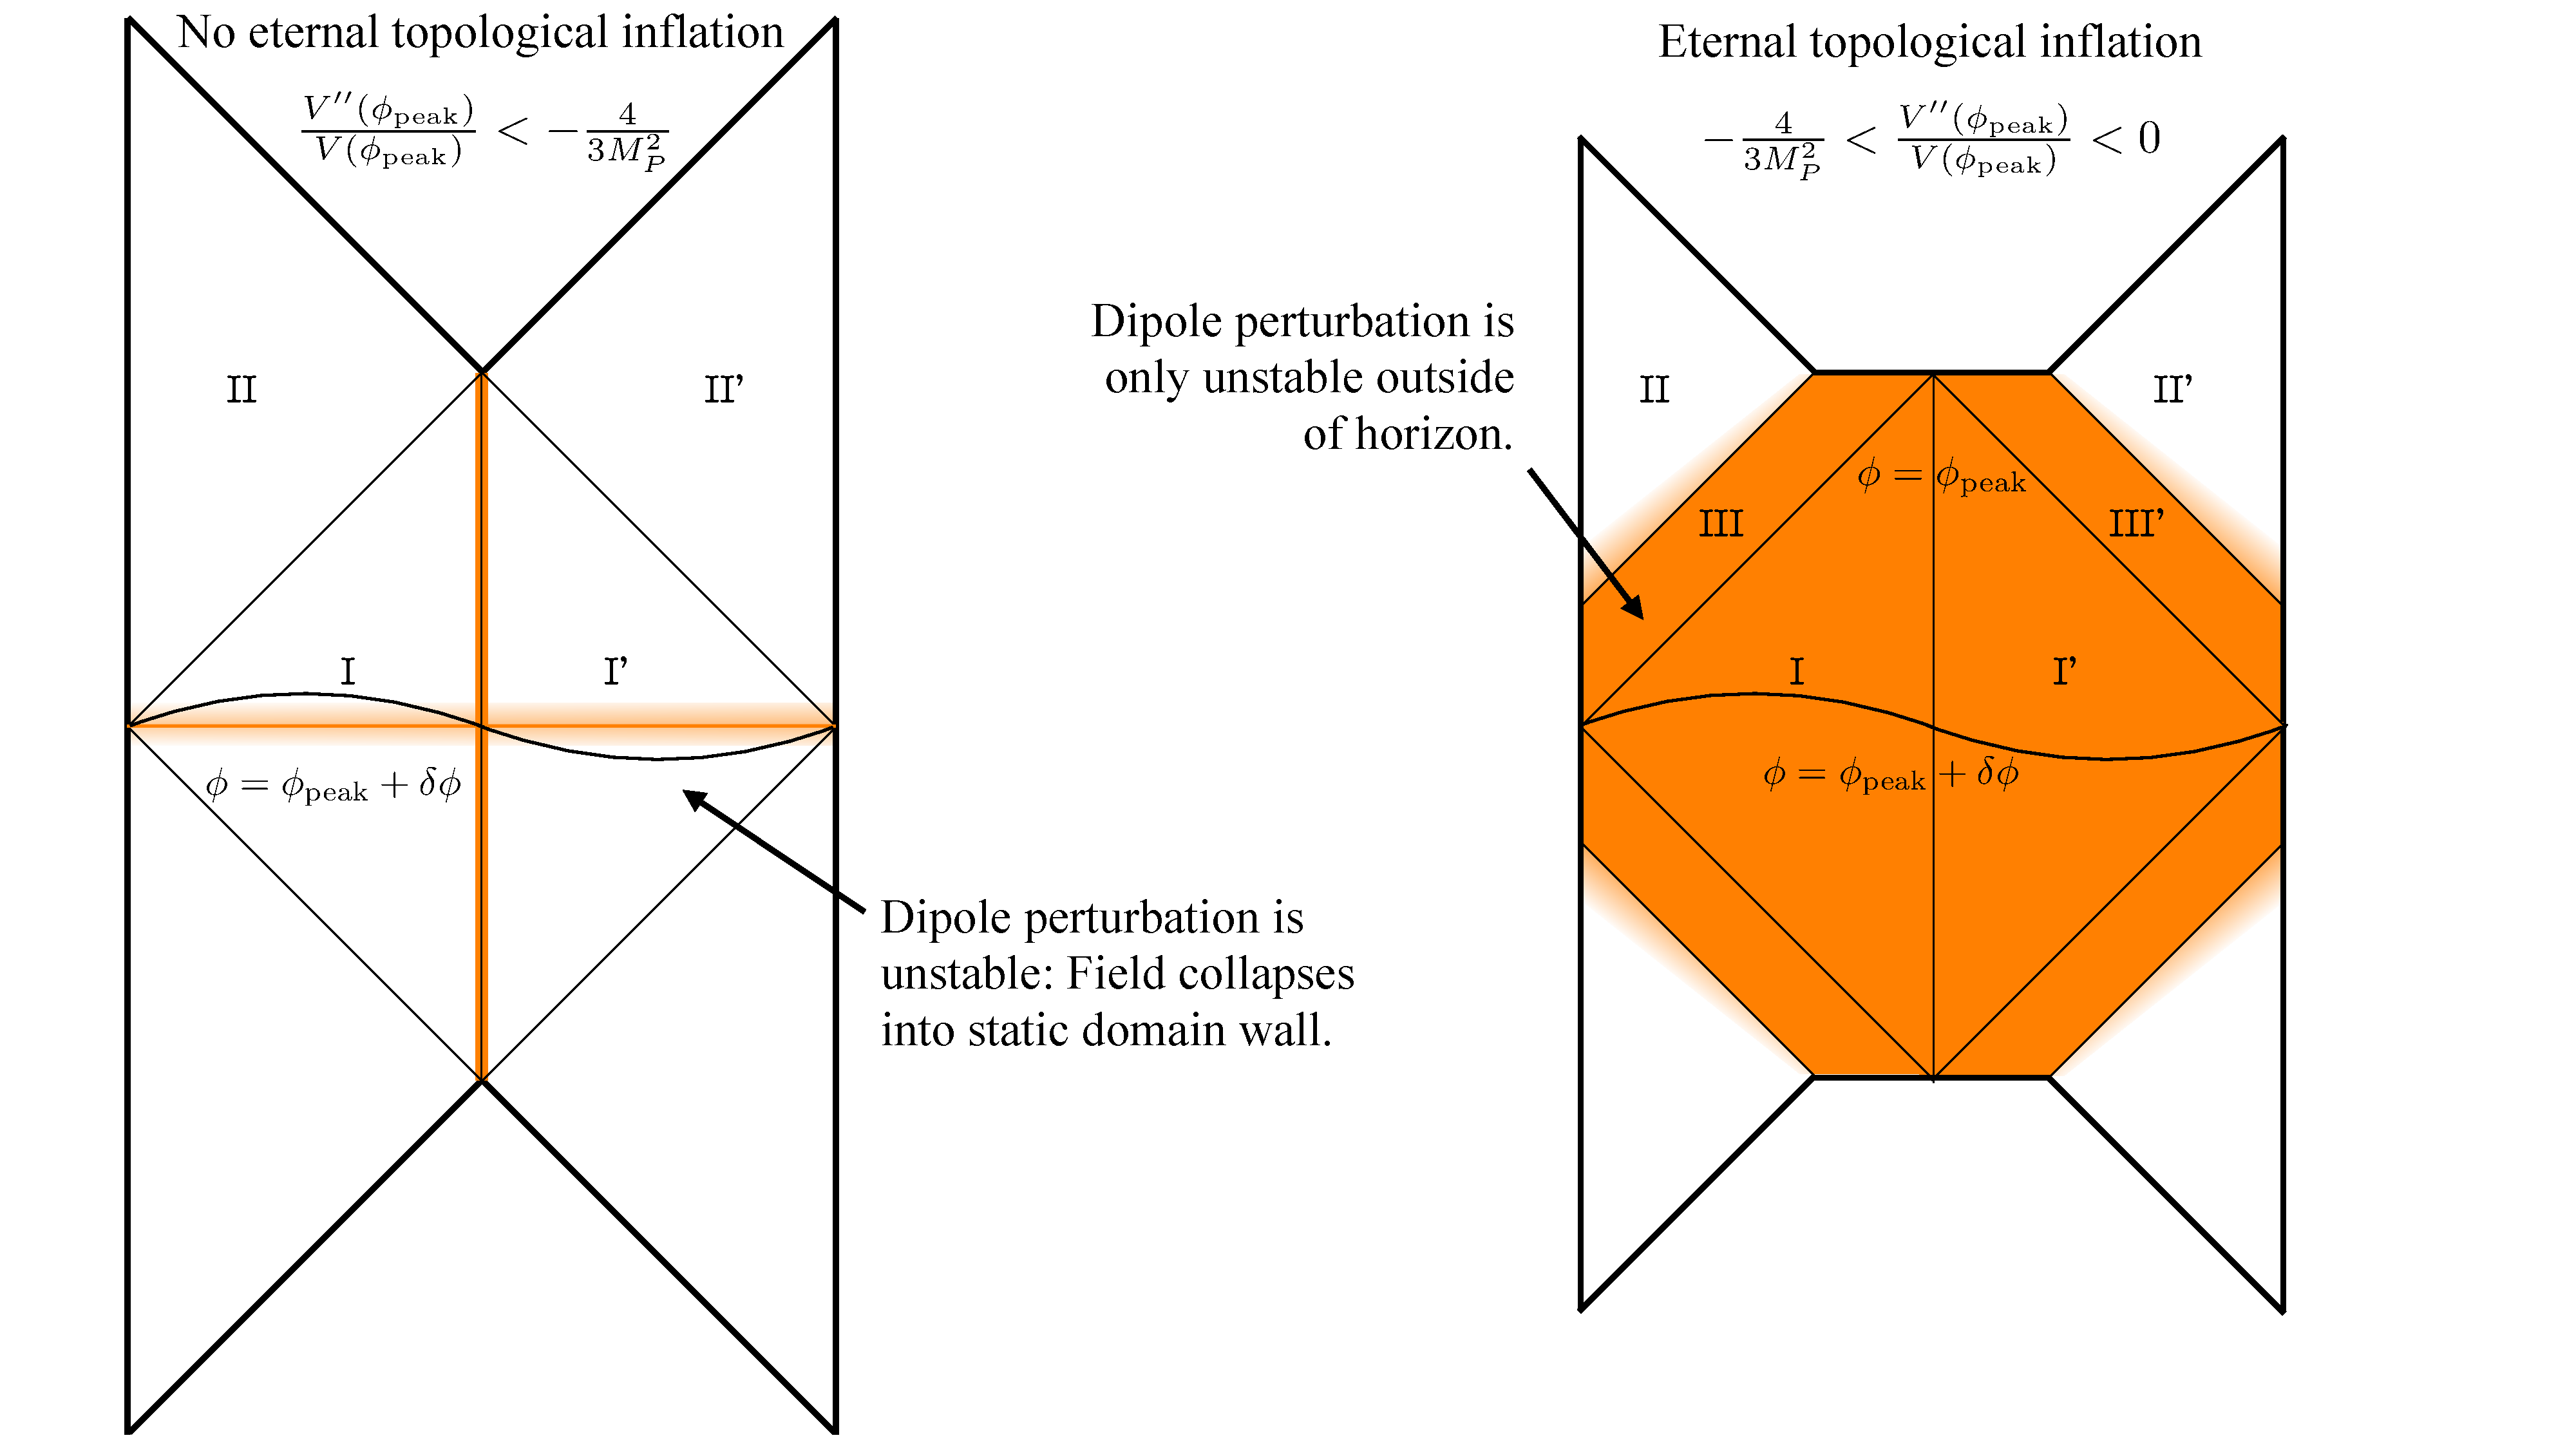
\includegraphics[width=1\textwidth]{figures/TEI}
\caption{{\bf Left:} When eternal topological inflation is not possible, any perturbation to the homogeneous $\phi(z) = \phi_{\rm peak}$ solution is unstable, and the field collapses into a finite thickness domain wall geometry.
{\bf Right:}  In the eternally inflating regime, a dipole perturbation cannot grow in the vicinity of the core, relaxing instead back to de Sitter space.  Thermalized regions II and II' do result from the perturbation, but are separated by a domain wall exponentially growing in thickness.}
\label{fig:TEI}
\end{center}
\end{figure}




The linearized equation of motion about $\phi = \phi_{\rm peak}$
\begin{align}
\frac{1}{\sqrt{-|g|}}\partial_\mu\left(\sqrt{-|g|}g^{\mu\nu}\partial_\nu\, \delta\phi\right) = V''(\phi_{\rm peak}) \delta\phi,
\end{align}
for static perturbation 
\begin{align}
\delta\phi = \sin(z/\ell_0),
\end{align}
takes the form
\begin{align}
-\frac{4}{\ell_0^2}\sin(z/\ell_0) = V''(\phi_{\rm peak})\sin(z/\ell_0).
\end{align}
Hence, eternal topological inflation exists when
\begin{align}
 -\frac{4}{3\MMp} \leq \frac{V''(\phi_{\rm peak})}{V(\phi_{\rm peak})} < 0.
\end{align}
For our model, this corresponds to
\begin{align}
f \geq \sqrt{3}\Mp/2.
\end{align}
Thus we can conclude that topological eternal inflation is impossible when $f < \sqrt{3}\Mp/2$,
since there exists an unstable perturbation, leading to finite thickness domain walls.




\section{Stochastic Eternal Inflation}\label{sec:stoc}
Another type of eternal inflation occurs when the monotonic classical rolling of the inflaton is persistently overwhelmed by its quantum fluctuations \cite{steinhardt1982,Vilenkin:1983xq,Linde:1983gd}.  
After each Hubble time, the physical spatial volume of an inflating Hubble volume grows by a factor of $e^3$.  If on average more than one daughter Hubble volume
experiences an uphill fluctuation, then stochastic eternal inflation inevitably occurs.


Although the slope at the inflection point is chosen large enough to forbid uphill fluctuations, the slope at the maximum of $V$ vanishes, and so could lead to stochastic eternal inflation \cite{Barenboim:2016mmw}.  
However all directions are downhill from the maximum, so the question is slightly more subtle, as we will show in the next subsection.

The classical evolution of the inflaton is given by the equation of motion
\begin{align}
\ddot \phi = -3 H \dot \phi - V'(\phi),
\end{align}
which has a ``slow-roll'' attractor solution
\begin{align}
\dot \phi \to \dot \phi_{\rm sr} = -\frac{V'(\phi)}{3 H}.
\end{align}
 The quantum fluctuation of the inflation field velocity in the Bunch-Davies state has amplitude
\begin{align}
\delta \dot \phi = \frac{H^2}{2\pi}.
\end{align} 
Eternal inflation occurs when the attractor solution for the classical (slow-roll) velocity
%\begin{align}
%\dot \phi = -2\MMp H'(\phi)
%\end{align}
is persistently smaller in magnitude than the Bunch-Davies quantum fluctuation.  In such a scenario, after a Hubble
time the scalar field is likely to have moved uphill in at least one of the $e^3\approx 20$ Hubble volumes produced during
a Hubble time, 

Thus we will define the region of field space satisfying
\begin{align}
\frac{\left| V'(\phi)\right|}{3 H} \lesssim  \frac{H^2}{2\pi}
\end{align}
as $\phi \in \Phi_{\rm ee}$.

Eternal inflation occurs when $\Phi_{\rm ee} > \frac{H}{2\pi}$, meaning the field does not fluctuate out of $\Phi_{\rm ee}$ in less than a Hubble time.


\subsection{near local maxima}\label{app:sei}
At the top of the potential the attractor velocity is zero, but a single point in field space cannot be relevant for eternal inflation\cite{Barenboim:2016mmw}.  
This is because the field velocity is bounded below by the quantum fluctuation.  
The fluctuating field exits any region smaller than $\Delta\phi = \frac{H}{2\pi}$ within a Hubble time.  



The eternal inflation region of the potential, defined as where classical motion along the attractor is subdominant, will be called $\Delta\phi_{\rm ee}$.  
It is given by the portion of the peak (or stationary inflection point) where $|\dot\phi_{\rm cl}| \leq \frac{H^2}{2\pi}$, i.e.,
\begin{align}
\left|V'(\phi)\right| \leq \frac{3 H^3}{2\pi}.
\end{align}

Thus stochastic eternal inflation can occur only if
\begin{align}
\Delta\phi_{\rm ee} \gtrsim \frac{H}{2\pi}.
\end{align}
For the potential whose local maximum resembles
\beq
V(\phi) \approx \Lambda^4\left[2 - \frac{\phi^2}{f^2}\right], \label{eq:Vp2}
\eeq
stochastic eternal inflation can occur for
\begin{align}
f > \Mp.
\end{align}
It is interesting that this is roughly the same bound as for the purely classical phenomenon of topological eternal inflation even though the argument here seems essentially quantum mechanical.  The reason
why quantum mechanics is effectively absent here is because we are comparing two effects that each scale with $\hbar$:  The region of the potential which supports uphill quantum fluctuations is proportional to $\hbar$ (using the quadratic approximation), and also the distance the inflaton moves in a Hubble time is proportional to $\hbar$.  Hence, the number of Hubble times before the field leaves this stochastic region is $\hbar$-independent, and thus appears classical.


\subsection{near an inflection point}
Since the local maximum cannot give rise to stochastic eternal inflation when $f \lesssim \Mp$, the last place we need to consider is near the inflection point. 
Note that for pure imaginary $\beta$, there is a false vacuum, and so unsurprisingly, stochastic eternal inflation exists near the inflection point for $\beta = 0$.  Such small
values of $\beta$ yield values of $n_s$ far too red to be compatible with observations (unless $f \gtrsim 10 \Mp$), as can be seen from figure \ref{fig:fbetaregion}. 
Existing constraints on the spectral index $n_s$ require $\beta > 0.01 f^2/\MMp$.  This rules out the possibility of stochastic eternal inflation for observationally viable regions of
parameter space, except in regions that already give rise to eternal topological inflation.



\section{Notes to ourselves}
\subsection{Goals}
\begin{enumerate}
\item Discuss the fine-tunings for small $f$ and for large $f$.  

\item Consider the possibility that $f$ is large, and the lack of tensors seen is due to a selection effect ?

\item Argue that interpreting the CMB is different in cases where there is a multiverse, vs. where the observable universe is not much smaller than the entire universe.  In particular, the multiverse provides an ensemble
that makes selection effects quantifiable.  For example, the cosmic-variance suppression of a tensor signal in the CMB could be a selection effect, and so ruling out $m^2\phi^2$ requires some additional data.  

%It is conceivable that selection effects that link the density of observers with scalar and tensor perturbations is peaked at certain comoving scales.  Then, future observations of tensors at solar system scales should find them.


\item Argue that the prior for a parameter value, $P(f)$, is dependent on considerations of simplicity or naturalness \cite{Musoke:2017frr}, monodromy, etc..

\item Argue that the prior for a parameter value, $P(f)$, might be strongly dependent on the existence of a multiverse or the solution to the measure problem.


\item Argue that the interpretations of tensor-mode data from solar-system scale experiments like BBO can better confirm or rule-out $m^2\phi^2$.  Unlike at CMB scales, new and independent solar-system-scale tensor modes can be measured continuously, providing a statement about primordial tensors whose confidence grows with time, rather than stagnating.  This allows for uncertainty in the prior $P(f)$ to become less of a hurdle in model selection.


\end{enumerate}

\subsection{Some questions}
 
 \begin{enumerate}
 \item
 \item 
 \end{enumerate}





\end{appendix}



\bibliography{observers}
  
\end{document}}

